\documentclass[11pt, twocolumn, twoside]{article}

\usepackage{graphicx}
\usepackage{amsmath, amssymb}
\usepackage{enumerate}
\usepackage{titleps}
\usepackage[top=1.25in,bottom=1in,right=0.75in,left=0.75in]{geometry}
\usepackage[parfill]{parskip}
\usepackage{titling}
\usepackage{hyperref}

\graphicspath{ {../images/} }

\newpagestyle{ruled}
{\setfoot{}{\thepage}{} \footrule}
\pagestyle{ruled}


\setlength{\droptitle}{-4em}   % This is your set screw
\posttitle{\par\end{center}\vskip 0.5em}


\title{6.867 Final Project Writeup} % Please change this
\date{}
\author {Vickie Ye and Alexandr Wang}


\begin{document}
\maketitle


\begin{abstract}
In this project, we compared different methods for facial expression recognition
using images from a Kaggle dataset released as a part of an ICML-2013 workshop
on representation learning.
We found that classification using features extracted manually from facial images
using principal component analysis yielded on average 40\% classification accuracy.
Using features extracted by facial landmark detection, we received on average 52\%
classification accuracy. However, when we used a convolutional neural network, we
received 65\% classification accuracy.
\end{abstract}

\section{Introduction}

In this project, we compared classification using features manually extracted from
facial images against classification using a convolutional neural net, which learns
the significant features of images through convolutional and pooling neural layers.
The two manual feature extraction methods we explored were principal component
analysis (PCA) and facial landmark detection.

\subsection{PCA}

In facial recognition, PCA is used in generating a low-dimensional representation of
face images as linear combinations of the first $k$ eigenfaces of training data.
Eigenfaces are the eigenvectors of the training data's covariance matrix; the first
eigenfaces are the vectors along which the training data shows the highest variance.
Thus, we can express a facial image vector, normally thousands of pixels, in terms of
the linearly independent basis of the first $k$ eigenvectors. 

\subsection{Facial Landmark Detection}

\subsection{Convolutional Neural Networks}

Convolutional neural networks (CNNs) are artificial neural networks that work particularly well for image data. The structure of CNNs exploits strong local correlation in the inputs. This is done by enforcing local connectivity between neurons of adjacent layers. The inputs of a hidden unit at a particular layer $n$ are some locally-connected subset of the units of the previous layer $n-1$, done in such a way that the input to layer $n$ represent some tile of the units of layer $n-1$, where all the tiles overlap.

In addition, CNNs utilize shared parameterizations (weight vector and bias) across layers. By constraining the same types of weights across layers, essentially replicating units across layers, allows for features to be detected regardless to their position in the initial input, making the network much more robust to real world image data. Additionally, by constraining multiple weights to be the same reduces the parameters to be learnt, increasing learning efficiency.

\section{Experimental Details}

\subsection{Datasets}

For this project, we primarily used a dataset released by Kaggle as a part of an
ICML-2013 workshop in representation learning.

\subsection

\subsection{Convolutional Neural Network}

To implement our convolutional neural network, we used Google's TensorFlow neural network library.

\subsubsection{Minimizing Overfitting}

Since the size of our training set was 28,709 labeled examples, and our neural net needed to go through many more than 28,000 examples to achieve convergence, we employed a few techniques to ensure that our convolutional neural net did not overfit to the training set.

First off, we implemented learning rate decay on our convolutional neural net, so that the learning rate decreased as it had been trained through more examples. We used exponential decay, so that that the learning rate decayed by a factor of $0.1$ after training through $1,200,000$ examples, and we had it decay in a step change manner as is visible in Figure \ref{fig:cnnloss}. We found that the step change learning rate decay worked better than a continuous exponential decay. This is probably because maintaining a high learning rate initially could ensure that the CNN was trained towards a good local optimum in fewer steps, whereas a steadily decreasing learning rate could limit the range of the neural network.

In addition, we implemented distortion of the images while training to artificially increase the size of our training set, and make our convolutional neural net more robust to slightly distorted inputs. We processed our images in a few different ways. We would crop our 48 by 48 pixel images to a 40 by 40 pixel box, centrally for model evaluation and randomly for training. Then we approximately whiten the photos, scaling the pixel values linearly so that they pixel values have a mean of 0 and a standard deviation of 1, essentially normalizing them. This ensures consistent inputs to our neural network.

For training in particular, we would do a few more distortions to artificially increase our training set. We randomly flipped the image from left to right, randomly distorted the image brightness, and 	randomly distorted the image contrast for each image. These changes to randomly distort the images greatly improved the performance of the model.

\begin{figure}
	\centering
	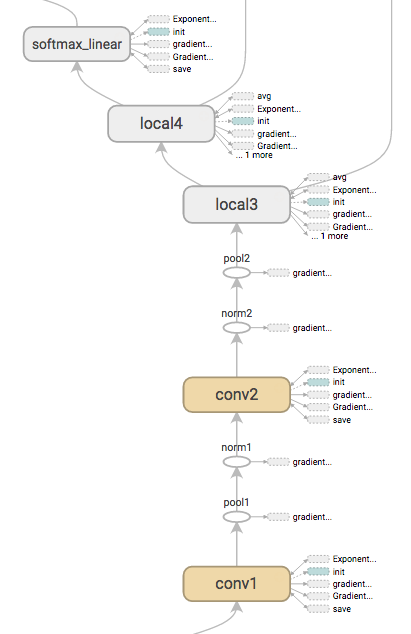
\includegraphics[width=3.25in]{inference_graph}
	\caption{TensorFlow computation graph for the neural network in the CNN we implemented, illustrating each of the layers.}
	\label{fig:inference}
\end{figure}

\section{Results and Analysis}

\begin{figure}
	\centering
	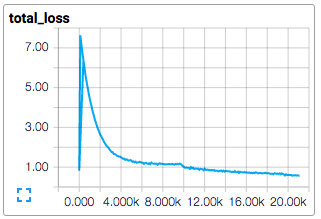
\includegraphics[width=3in]{total_loss}
	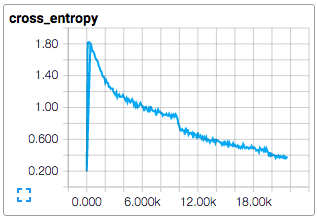
\includegraphics[width=3in]{cross_entropy}
	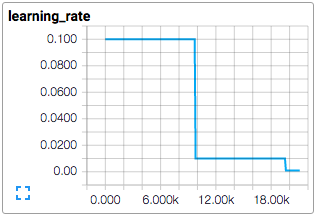
\includegraphics[width=3in]{learning_rate}
	\caption{The total loss, cross entropy, and learning rate of the convolutional neural net over time.}
	\label{fig:cnnloss}
\end{figure}

\begin{figure}
	\centering
	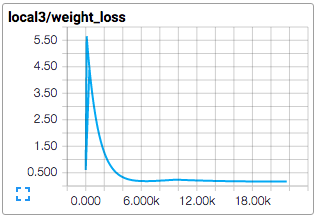
\includegraphics[width=3in]{local3_loss}
	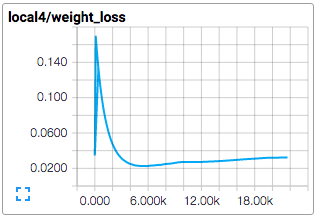
\includegraphics[width=3in]{local4_loss}
	\caption{The loss on the local3 layer and local4 layer over time in the convolutional neural net.}
	\label{fig:layer_loss}
\end{figure}


\begin{thebibliography}{9}
\bibitem{Lawrence}
Lawrence, S.; Giles, L.; Tsoi, A. C.; Back, A. D. (1997)
``Face Recognition: A Convolutional Neural-Network Approach"
\textit{Neural Networks, IEEE transactions on} 8 (1):98-113
\bibitem{Matsugu}
Matsugu, M.; Mori, K.; Mitari Y.; Kaneda Y. (2003)
``Subject independent facial expression recognition with robust face detection using a convolutional neural network"
\textit{Neural Networks} 16 (5):555-559
\end{thebibliography}

\end{document}
